\subsection{Sensitivity to Resolved Schedule Parameters}
\label{sec:eval:sensitivity}

\begingroup
\setlength{\intextsep}{8pt}
\begin{figure}[t]
    \centering
    \begingroup
    % Keep these fills identical to GROUP_BACKGROUNDS in
    % plot_scripts/plot_resolved_tiling_sensitivity.py.
    \definecolor{controlflowbg}{HTML}{F8D7DA}
    \definecolor{addresscalcgbg}{HTML}{D9EAD3}
    \definecolor{mmschedulebg}{HTML}{DDEBF7}
    \newcommand{\controlmath}[1]{{\setlength{\fboxsep}{1.0pt}%
        \colorbox{controlflowbg}{\strut\ensuremath{#1}}}}
    \newcommand{\addressmath}[1]{{\setlength{\fboxsep}{1.0pt}%
        \colorbox{addresscalcgbg}{\strut\ensuremath{#1}}}}
    \newcommand{\schedulemath}[1]{{\setlength{\fboxsep}{1.0pt}%
        \colorbox{mmschedulebg}{\strut\ensuremath{#1}}}}
    \newcommand{\auxfn}[1]{{\sffamily\bfseries #1}}
    \newcommand{\controlgroup}[1]{{\setlength{\fboxsep}{1.5pt}%
        \colorbox{controlflowbg}{\parbox{0.91\linewidth}{#1}}}}
    \newcommand{\addressgroup}[1]{{\setlength{\fboxsep}{1.5pt}%
        \colorbox{addresscalcgbg}{\parbox{0.91\linewidth}{#1}}}}
    \newcommand{\schedulegroup}[1]{{\setlength{\fboxsep}{1.5pt}%
        \colorbox{mmschedulebg}{\parbox{0.91\linewidth}{#1}}}}

    \begin{minipage}[t]{0.405\linewidth}
        \fontsize{5.45}{6.05}\selectfont
        \setlength{\fboxsep}{3pt}
        \fcolorbox{black!30}{white}{%
        \parbox[t][0.72in][t]{0.92\linewidth}{%
            \centering
            \textbf{(a) D-Attn \(\mathrm{Query}\times\mathrm{Key}^{\mathsf T}\)}\par
            \vspace{1pt}
            \(\displaystyle
            \mathrm{Output}_{b,h}
              =\mathrm{Query}_{b,h}\mathrm{Key}_{b,h}^{\mathsf T}
            \)\par
            \vspace{1pt}
            \raggedright
            \(\mathrm{Query}_{b,h}:[1,D_{head}]\): Query row of attention
            head \(h\) for request \(b\) in the batch.\par
            \(\mathrm{Key}_{b,h}:[T_b,D_{head}]\): cached Key rows of
            attention head \(h\) for request \(b\) in the batch.\par
            \(\mathbf{T}=[T_0,\ldots,T_{B-1}]\): per-request KV lengths
            (runtime input).
        }}\par
        \vspace{3pt}
        \fontsize{5.05}{5.50}\selectfont
        \fcolorbox{black!30}{white}{%
        \parbox[t][1.15in][t]{0.92\linewidth}{%
            \centering
            \textbf{(b) Representative schedule parameters for
                \(\mathrm{Query}\times\mathrm{Key}^{\mathsf T}\)}(34 total)\par
            \vspace{2pt}
            \raggedright
            \controlgroup{%
                \centering
                \textbf{Control logic (6 total)}\par
                \raggedright
                \(T_N\): Key rows in one output tile.\\
                \(P\): Key rows in one cache page.\\
                \(T_D\): Key columns in one narrow load.
            }\par
            \vspace{1pt}
            \addressgroup{%
                \centering
                \textbf{Per-core tile dimensions/addressing
                (14 total)}\par
                \raggedright
                \(M_c\): Output-row extent assigned to one core.\\
                \(K_c\): Reduction-column extent assigned to one core.
            }\par
            \vspace{1pt}
            \schedulegroup{%
                \centering
                \textbf{Core-loop scheduling/memory resources
                (14 total)}\par
                \raggedright
                \(N_c\): Number of active compute cores.\\
                \(n_K\): Number of Key buffers.
            }
        }}
    \end{minipage}\hfill
    \begin{minipage}[t]{0.575\linewidth}
        \fontsize{4.80}{5.20}\selectfont
        \setlength{\fboxsep}{3pt}
        \fcolorbox{black!30}{white}{%
        \parbox[t][2.10in][t]{0.94\linewidth}{%
            \centering
            \textbf{(c) Tiled BMM pseudocode for
                \(\mathrm{Query}\times\mathrm{Key}^{\mathsf T}\)}\par
            \vspace{2pt}
            \raggedright
            \ttfamily
            \begin{tabular}{@{}>{\color{black!55}}r@{\hspace{3pt}}l@{}}
             1 & \textbf{function} \auxfn{BMM}(Query, Key, \(\mathbf{T}\);
                 \(\controlmath{T_N},\controlmath{P},\controlmath{T_D},
                 \addressmath{M_c},\addressmath{K_c},
                 \schedulemath{N_c},\schedulemath{n_K}\)) \\
             2 & \quad configure \(\schedulemath{N_c}\) cores and
                 \(\schedulemath{n_K}\) Key buffers \\
             3 & \quad\textbf{parallel for} \(c=0,\ldots,\schedulemath{N_c}-1\) \\
             4 & \quad\quad\textbf{for} tile \(\tau\) with
                 \(\controlmath{T_N}\) Key rows \(\times\)
                 \(\addressmath{K_c}\) columns assigned to core \(c\) \\
             5 & \quad\quad\quad \textit{// \(n_0\): first Key row;
                 \(k_0\): first reduction column; \(T_b\): request \(b\)'s KV length} \\
             6 & \quad\quad\quad
                 \((b,h,n_0,k_0)\leftarrow
                 \text{\auxfn{TileOffset}}(\tau;\addressmath{M_c},
                 \controlmath{T_N},\addressmath{K_c},\mathbf{T})\) \\
             7 & \quad\quad\quad
                 \(n\leftarrow\min(\controlmath{T_N},T_b-n_0)\) \\
             8 & \quad\quad\quad \textbf{for} \((p,r,u)\) in
                 \auxfn{PageFragments}\((\mathrm{Key},b,n_0,n;\controlmath{P})\) \\
             9 & \quad\quad\quad\quad\textbf{if}
                 \(\controlmath{T_N}=\controlmath{P}\) \\
            10 & \quad\quad\quad\quad\quad
                 one-copy load Key\([p,r:r+u,h,k_0:k_0+\addressmath{K_c}]\)
                 \(\rightarrow\mathrm{KeyBuf[next(}\schedulemath{n_K}\mathrm{)]}\) \\
            11 & \quad\quad\quad\quad\textbf{else}
                 \(\;(\controlmath{T_N}\ne\controlmath{P})\) \\
            12 & \quad\quad\quad\quad\quad\textbf{for}
                 \(d_0=k_0,k_0+\controlmath{T_D},\ldots,
                 k_0+\addressmath{K_c}\) \\
            13 & \quad\quad\quad\quad\quad\quad
                 append load Key\([p,r:r+u,h,d_0:d_0+\controlmath{T_D}]\)
                 \(\rightarrow\mathrm{KeyBuf[next(}\schedulemath{n_K}\mathrm{)]}\) \\
            14 & \quad\quad\quad
                 load Query\([b,0,h,k_0:k_0+\addressmath{K_c}]\)
                 \(\rightarrow\mathrm{QueryBuf}\) \\
            15 & \quad\quad\quad Output\(_{\rm tile}\mathrel{+}=\)
                 \auxfn{MMAD}(QueryBuf, KeyBuf)
            \end{tabular}
            \vspace{3pt}\par
            \rmfamily
            \auxfn{TileOffset}: maps tile \(\tau\) to start coordinate
            \((b,h,n_0,k_0)\): request, head, Key row, and reduction column.\par
            \auxfn{PageFragments}: resolves \(n\) logical Key rows through the
            page table as non-crossing fragments \((p,r,u)\).\par
            \auxfn{MMAD}: multiplies QueryBuf by KeyBuf and accumulates the
            partial result into Output\(_{\rm tile}\).
        }}
    \end{minipage}

    \caption{Tiled D-Attn BMM. Panel (b) lists seven representative
    schedule parameters; the three groups contain 6, 14, and 14 schedule
    parameters in total. Matching backgrounds in panel (c) mark their use
    sites and correspond to the groups evaluated in
    \autoref{fig:eval:constant-sensitivity}.}
    \Description{Three panels. Panel (a) defines the per-request Query--Key
    multiplication, explains the Query and Key tensors for request and head
    indices, and defines the runtime array of per-request KV lengths. Panel
    (b) lists seven representative schedule parameters and gives total
    counts of 6, 14, and 14 schedule parameters for Control logic, Per-core tile
    dimensions/addressing, and Core-loop scheduling/memory resources,
    respectively. Panel (c) takes all seven schedule
    parameters as inputs and shows core configuration, per-core tile indexing,
    page-aware Key loading with separate T-N-equals-P and T-N-not-equals-P
    paths, and the final tiled matrix multiplication.}
    \label{fig:resolved-tiling-code}
    \endgroup
\end{figure}


\begin{figure}[t]
	\centering
	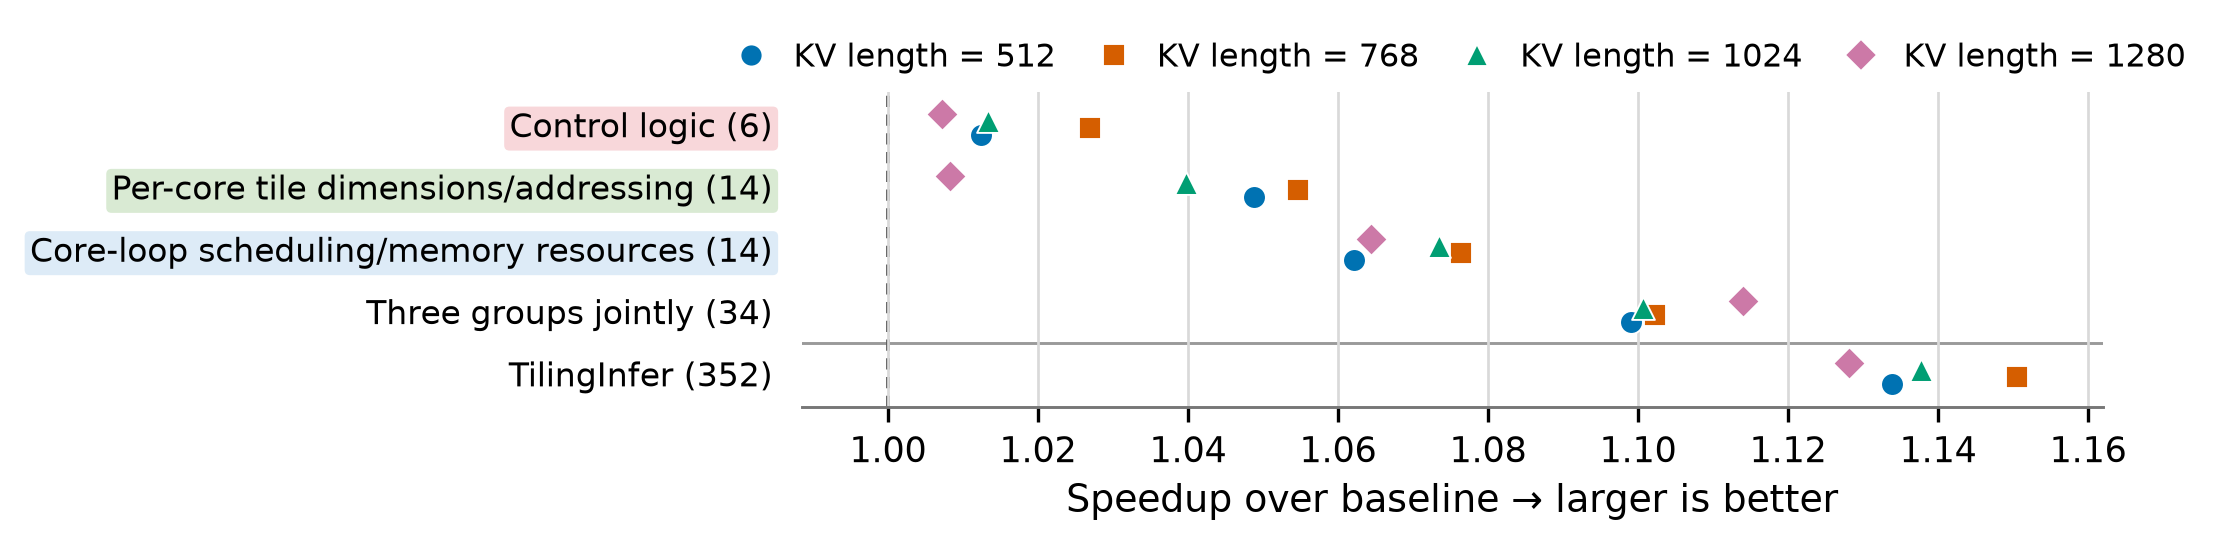
\includegraphics[width=0.85\textwidth]{figures/evaluation/op-speedup/resolved_constant_sensitivity.pdf}
	\caption{Sensitivity to resolved schedule parameters across runtime
	shapes. Numbers in parentheses give the number of specialized schedule
	parameters. Each point shows the speedup at one KV length; the first three
	label backgrounds match the groups in
	\autoref{fig:resolved-tiling-code}.}
	\Description{Point plot of speedup over Baseline for Control logic with 6
	specialized parameters, Per-core tile dimensions/addressing with 14,
	Core-loop scheduling/memory resources with 14, the three groups jointly
	with 34, and TilingInfer with 304.
	Each row contains separate points for KV lengths 512, 768, 1024, and 1280,
	and no error bars.}
	\label{fig:eval:constant-sensitivity}
\end{figure}
\endgroup

{\color{blue}%
This section analyzes whether specializing different groups of schedule parameters yields different benefits: can one group provide a substantially larger gain than the others?
\par}

{\color{blue}%
For D-Attn, $\mathrm{Query}_{b,h}\mathrm{Key}_{b,h}^{\mathsf T}$ multiplies the Query row of request $b$ and attention head $h$ by its cached Key rows, while $\mathbf{T}$ stores each request's KV length. Its 34 schedule parameters form Control logic (6), Per-core tile dimensions/addressing (14), and Core-loop scheduling/memory resources (14). Control logic covers the branches and loop bounds that select how Key data are loaded. Per-core tile dimensions/addressing specifies how much work each core owns and maps tile indices to tensor addresses. Core-loop scheduling/memory resources controls how tiles are assigned to active cores and how on-chip buffers are allocated and reused inside the core loop. \autoref{fig:resolved-tiling-code}(b) lists seven representative examples. In panel (c), $T_N$ and $K_c$ split Key rows and reduction columns into tiles, while $M_c$ and $N_c$ distribute the tiles to cores. TileOffset uses these extents and $\mathbf{T}$ to recover $(b,h,n_0,k_0)$, the tile's starting coordinate. The schedule parameters $T_N$, $P$, and $T_D$ select one page-aligned load or several narrow page-table loads, while $n_K$ selects the Key buffer. BMM then loads the matching Query slice and computes the tile.
\par}

{\color{blue}%
Overall, \autoref{fig:eval:constant-sensitivity} shows that specialization value depends more on a parameter's use site than on parameter count. Across KV lengths 512--1280, the 14 Core-loop scheduling/memory-resource parameters achieve the largest isolated geometric-mean speedup, 1.07$\times$, by configuring per-core work and Key-buffer resources on the inner BMM path. The 14 Per-core tile dimension/addressing parameters reach 1.04$\times$, while the 6 Control-logic parameters reach 1.02$\times$. Thus, count alone poorly predicts specialization value.
\par}

{\color{blue}%
The three isolated gains sum to 12.2\%, whereas jointly specializing all 34 parameters yields 1.10$\times$ (10.4\%), or 85.0\% of that sum, indicating interaction and diminishing returns. TilingInfer specializes 304 stable parameters and reaches 1.14$\times$. Although the 34 $\mathrm{Query}\times\mathrm{Key}^{\mathsf T}$ parameters comprise only 11.0\% of these fields, they recover 75.0\% of the full gain; the remaining 270 add only 3.4 percentage points. Because these 34 parameters control D-Attn's core BMM in \autoref{fig:resolved-tiling-code}(c), specializing its hot-path address and control flow is more valuable than resolving constants on colder paths.
\par}
